\documentclass{article}

 %%%  Layout da folha e margens
\usepackage{geometry}[a4paper, left=3cm, top=3cm, right=2cm, bottom=2cm]

\usepackage{graphicx} % Required for inserting images

%%% Pacote para criar ambientes para alinhamento do texto 
\usepackage{ragged2e}

%%% Pacote para adicionar seções aos ambientes flutuantes
\usepackage{threeparttable}
\usepackage{caption}

%%% Fontes e simbolos matemáticos
\usepackage{amsmath}
\usepackage{amsfonts}
\usepackage{setspace}

%%% Definição do idioma
\usepackage[portuguese]{babel}
\usepackage{inputenc}
\selectlanguage{portuguese}

%%% Pacote para subfiguras
\usepackage{subfigure}


%%% Pacote para utilização de pretty-print para códigos - Lua
\usepackage{listings}
\lstset{
  language={[5.0]Lua},
  frame=single,
  breaklines=true,
}


%%% Command for numbering individual equations in align environment
\newcommand\numberthis{\addtocounter{equation}{1}\tag{\theequation}}

%%% Criação de um ambiente flutuante para quadros anáologo a figuras e tabelas
\usepackage{newfloat}
\DeclareFloatingEnvironment[
  fileext=loq,
  listname={Lista de Quadros},
  name=Quadro,
  placement=ht,
  within=section
]{quadro}



\title{\textbf{Water Dam Exercise} | 
CST-323 Introduction to Earth System Modelling}
\author{Luiz Gabriel Silva \\ Thaís Pereira de Medeiros}
\date{Julho 2023}


\begin{document}

\onehalfspacing
\maketitle

\section{Enunciado}

In the year of 1950, a given city has 100,000 inhabitants. A dam with a capacity of 5,000,000,000m³ of water produces hydroelectric energy for the whole city. In the region, two rainy seasons take place in each year. In the first season, the rains add 2,000,000,000m³ of water to the dam, while in the second they add 1,500,000,000m³. In the beginning of 1950, the dam is full and each inhabitant consumes on average 10kWh of energy per month. Each kWh of energy requires 100m³ of water to be produced. The consumption of energy increases an average of 5\% per inhabitant each year. Develop a model to investigate future scenarios for the dam. For each of the scenarios below, how long will it take until the dam is not able to provide all the energy required by the city?

1) If nothing else happens.

2) If the turbines would require only 80m³ of water to generate 1kWh.

3) If the consumption growth falls by half.

4) If the overall rain falls by half from 1970 onwards.

5) If the scenarios (2), (3), and (4) take place.

\section{Exploração prévia}

\subsection{Crescimento da taxa de consumo}

Observe que o consumo de energia por habitante da cidade no ano $x$ ($k_x$, onde $x \geq 1950$], pode ser calculada inicialmente do seguinte modo:

\begin{align*}
    k_{1950} &= k \\
    k_{1951} &= k_{1950} + k_{1950} \times \alpha \\
    \vdots \\
    k_{x} &= k_{x - 1} + k_{x - 1} \times \alpha
\end{align*}
onde $k_x$ é o consumo em um determinado ano e $\alpha$ é a taxa de crescimento do consumo.

Fazendo as devidas substituições, obtém-se a seguinte fórmula para o cálculo de $k_x$:
\begin{equation}
    k_x = k(1 + \alpha)^{x - 1950}
\end{equation}

A quantidade mensal ($Q_x^m$) de água consumida pela cidade para gerar energia em um dado ano $x$ pode ser obtida do seguinte modo:
\begin{equation}
\label{eq: consumo_mensal}
    Q_x^m = \beta N k_x \Rightarrow  Q_x^m = \beta N k(1 + \alpha)^{x - 1950},
\end{equation}
onde, $N$ é o número de habitantes da cidade e $\beta [m^3/KWh]$ é a taxa de conversão de volume de água em energia.

Como $k_x$ é constante ao longo de um ano, o consumo anual de água no ano $x$ é:
\begin{equation}
\label{eq: consumo_anual}
    Q_x^y = 12 Q_x^m \Rightarrow Q_x^y = 12\beta N k(1 + \alpha)^{x - 1950}.
\end{equation}

Embora não seja possível simular resolver o problema utilizando apenas as Equações \ref{eq: consumo_mensal} e \ref{eq: consumo_anual}, elas nos ajudam a obter alguma intuição sobre a dinâmica do volume de água na represa.

\subsection{Estudos de caso}

\subsubsection{Ausência de chuvas}

A primeira situação que podemos considerar, e a mais simples, é a situação na qual há ausência de chuvas e represa se encontra com o volume máximo de água ($V_{max})$. Nesse caso, o volume ($V_j)$ de água na represa após o j-ésimo ano é:
\begin{equation}
    V_j = V_{max} - \sum_{i=0}^{j} Q_{i + 1950}^y
\end{equation}
Desse modo:
\begin{align*}
    \sum_{i=0}^{j} Q_{i + 1950}^y &= \sum_{i=0}^{j} 12\beta N k(1 + \alpha)^{i} \\
                                  &= 12\beta N k\sum_{i=0}^{j} (1 + \alpha)^{i} = 12\beta Nk \left[ \frac{(1 + \alpha)^{j} - 1}{\alpha}\right]
\end{align*}

Cabe observar que, estamos desprezando o primeiro termo da progressão geométrica na soma acima, isso foi feito para garantir a seguinte interpretação dos resultados. Para $j = 0$, ou seja, nenhum tempo transcorrido, a quantidade consumida de água da represa será $0 m^3$, transcorrido um ano ($j = 1$), a quantidade de água será o volume inicial menos o volume consumido em 1950, e assim por diante. Como $V_j \geq 0$, temos que:
\begin{align*}
    V_{max} &\geq \sum_{i=0}^{j} Q_{i + 1950}^y \\
    &\Downarrow\\ 
    V_{max} &\geq 12\beta Nk \left[ \frac{(1 + \alpha)^{j} - 1}{\alpha}\right] \\
    &\Downarrow \\
    j &\leq \frac{\log{\left[ \frac{\displaystyle \alpha V_{max}}{12\beta Nk}\right]} + 1}{\displaystyle \log{(1 + \alpha)}} \numberthis \label{eq: anos_cota_inferior}
\end{align*}

Utilizando a Equação \ref{eq: anos_cota_inferior} podemos calcular o número de anos para esgotamento da represa considerando vários cenários. Os resultados dos cálculo podem ser vistos na Tabela \ref{tab:cotas_ano_esgotamento}. Esses resultados indicam que, não há possibilidade da água se esgotar antes de aproximadamente quatro ou cinco anos, a depender da eficiência da conversão de água em energia. Esses resultados também serão utilizados para testar a validade da implementação do modelo. 

\begin{table}[ht!]
    \centering
    \caption{Ano de esgotamento do volume de água da represa, variando a taxa de crescimento de consumo de energia da população ($\alpha$) e a quantidade de água necessária para produção de energia ($\beta$). Os demais parâmetros foram utilizados com valores fixos: $N = 1e5$, $k = 10$ e $V_{max}^{rain} = 3.5e9$.}
    \label{tab:cotas_ano_esgotamento}
    \begin{tabular}{lcccccc}
        \hline
             & \multicolumn{2}{l}{Ausência de chuvas} & \multicolumn{2}{l}{Cotas inferiores} & \multicolumn{2}{l}{Cotas superiores} \\ \cline{2-7} 
             & \multicolumn{2}{c}{$\alpha$}              & \multicolumn{2}{c}{$\alpha$}            & \multicolumn{2}{c}{$\alpha$}            \\ \cline{2-7} 
        $\beta$ & 0.025               & 0.05               & 0.025              & 0.05              & 0.025              & 0.05           \\ \hline
        80      & 1954                & 1954               & 2007               & 1981              & 2018               & 1987            \\
        100     & 1954                & 1953               & 1997               & 1975              & 2010               & 1982            \\ \hline
    \end{tabular}
    {\flushleft Fonte: os autores. \par}
\end{table}



\subsubsection*{Cotas inferiores}

Embora possamos utilizar os valores obtidos anteriormente como cotas inferiores, podemos obter cotas melhores. Há duas situações extremas, na primeira, as chuvas estão concentradas em um único mês, e na segunda, as chuvas estão distribuídas uniformemente durante o ano. A primeira situação, dificulta o aproveitamento da água da chuva, uma vez que a represa tem capacidade limitada, e é a condição que resulta no menor tempo necessário para esgotamento da água da represa. Nesse caso, observe que a água da represa só se esgotará após o consumo anual superar o volume de chuvas, desse modo:

\begin{equation}
    V_{max}^{rain} \leq Q_x^y
\end{equation},
onde $V_{max}^{rain}$ é volume máximo acumulado de chuvas no ano. Assim:

\begin{align*}
     V_{max}^{rain} &\leq 12\beta N k(1 + \alpha)^{x - 1950} \\
                             &\Downarrow \\
    x                        &\geq \frac{\log{\left[ \frac{\displaystyle V_{max}^{rain}}{12\beta Nk}\right]}}{\displaystyle \log{(1 + \alpha)}} + 1950 \numberthis \label{eq: anos_cota_inferior}
\end{align*}
Duas observações, a primeira é que $x \in \mathbb(R)$, e para definirmos um ano mínimo, utilizaremos o menor interior por baixo de $x$, $\lfloor x \rfloor$. A segunda é que podemos melhorar um pouco essa cota, dado que nessa condição em que o consumo anual iguala o volume de água da chuva, ainda restará o volume água da represa a ser consumido. Desse modo, a cota inferior para esgotamento da água da represa ($X_{inf})$ será:
\begin{equation}
\label{eq: cota_inferior}
    X_{inf} = \lfloor x + j  \rfloor
\end{equation},
onde $j$ é o tempo necessário para esgotamento da represa na ausência de chuvas. As cotas calculadas a partir da equação \ref{eq: cota_inferior} estão apresentados na Tabela \ref{tab:cotas_ano_esgotamento}.


\subsubsection*{Cotas superiores}
Para obter cotas superiores, observe que após o consumo igualar o volume agregado da quantidade de chuvas e do consumo no ano de 1950 (ano de referência), voltamos a condição similar a situação de ausência de chuvas. A diferença é que nesse caso o processo não se inicia com a represa completa. Esse detalhe piora a estimativa da cota superior, não a invalida. Desse modo:

\begin{align*}
    Q_{1950}^y + V_{max}^{rain} &\geq Q_x^y \\
                                &\Downarrow \\
    Q_{1950}^y + V_{max}^{rain} &\geq 12\beta N k(1 + \alpha)^{x - 1950} \\
                                &\Downarrow \\
    x                           &\leq \frac{\log{\left[ \frac{\displaystyle Q_{1950}^y + V_{max}^{rain}}{12\beta Nk}\right]}}{\displaystyle \log{(1 + \alpha)}} + 1950 \numberthis \label{eq: anos_cota_superior}
\end{align*}
De modo análogo ao caso anterior:
\begin{equation}
\label{eq: cota_superior}
    X_{sup} = \lceil x + j  \rceil
\end{equation}
As cotas calculadas a partir da equação \ref{eq: cota_superior} estão apresentados na Tabela \ref{tab:cotas_ano_esgotamento}.

\subsection*{Modelos}

O modelo criado para simulação da dinâmica do sistema de interesse for desenvolvido em três etapas, com níveis de complexidade crescentes em relação a representação da chuva. O modelo criado na primeira etapa considera a chuva total distribuída igualmente ao longo do ano, e foi utilizada como base para as próximas etapas e para testes. O modelo criado na segunda etapa, faz distinção entre duas estações chuvosas, conforme descrito no enunciado. Foi adotado o período de seis meses para cada estação, com chuvas uniformemente distribuída entre os meses da mesma estação. Na terceira etapa, foram utilizados valores mensais de chuva distintos para cada mês do ano. A distribuição de chuvas foi derivada a partir da normal climatológica (médias de 30 anos - período 1991-2020) de pluviometria da cidade de São Paulo-SP (Figura \ref{fig:distribuicao_chuva}).

\begin{figure}
    \centering
    \caption{Distribuição de Chuvas ao longo do ano}
    \label{fig:distribuicao_chuva}
    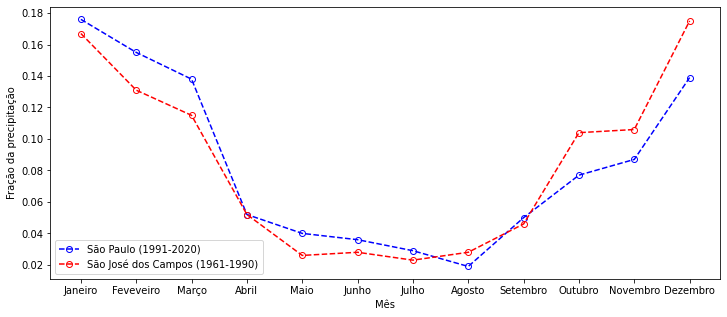
\includegraphics[width=0.9\textwidth]{imagens/pluviometria.png}
    {\flushleft Fonte: os autores, utilizando dados pluviométricos disponibilizados pelo Instituto Nacional de Meteorologia - INMET. \par}
\end{figure}

Cabe notar que a distribuição de chuvas utilizada é um pouco diferente da distribuição do enunciado, onde aproximadamente 57,15\% e 42,85\% do total de chuvas ocorrem na primeira e na segunda estações chuvosas, respectivamente. Considerando os dados para a cidade de São Paulo e agosto como início da segunda estação chuvosa no ano, aproximadamente 64,7\% e 35.3\% das chuvas ocorrem na primeira e na segunda estações chuvosas, respectivamente. Considerando as cotas superiores e inferiores obtidas, bem como os resultados das simulações com chuvas uniformemente distribuídas ao longo do ano e longo de uma estação, essa diferença aparentemente não deve provocar alterações importantes nos resultados.

%\subsubsection*{Códigos}
%
%\begin{quadro}
%\caption{Código da função para atualização do volume de água na represa}
%\begin{threeparttable}[t]
%    \begin{lstlisting}
%    execute = function(model)
%        model.waterVol = model.waterVol - model.nInhab * model.energyCons * model.waterEnergyRatio + model.seasonRain
%
%        if model.waterVol > model.damCap then
%            model.waterVol = model.damCap
%        elseif model.waterVol < 0 then
%            model.waterVol = 0
%        end
%    end
%    \end{lstlisting}
%    \begin{tablenotes}[flushleft]
%        \item[] Fonte: os autores.
%    \end{tablenotes}
%\end{threeparttable}
%\end{quadro}
%
\subsubsection*{Testes}

Foram obtidos resultados muito próximos para as simulações dos modelos produzidos (Figura \ref{fig:comparacao_resultados}).

\begin{figure}[ht!]
    \centering
    \caption{Comparação entre as simulações dos modelos}
    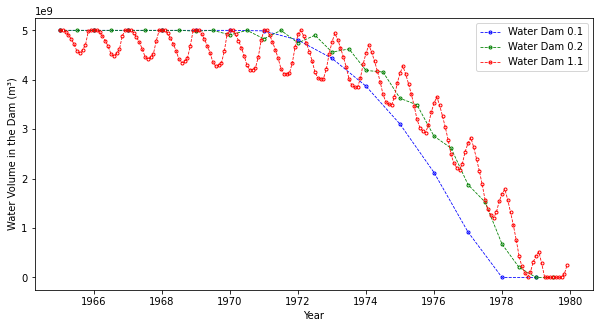
\includegraphics[width=0.9\textwidth]{imagens/model_comp.png}
    \label{fig:comparacao_resultados}
    {\flushleft Fonte: os autores.\par}
\end{figure}


\subsection*{Resultados}


Foram realizadas cinco simulações, numeradas de 1 a 5, que correspondem as situações descritas no enunciado (Figura \ref{fig:resultados}). Como podemos notar, a longo prazo a melhor estratégia para prolongamento da vida útil da represa é a economia de energia por habitante (ou qualquer outra estratégia que reduza a taxa de crescimento do consumo médio por 100 mil habitantes). A melhoria na eficiência do processo não garante muito tempo extra, em relação a situação de referência (Sim 1). Outra característica interessante é que a mudança da situação de represa cheia para represa vazia é relativamente repentina, em todas as situações, assim que o nível anual começa a baixar, rapidamente o volume de água se esgota.

\begin{figure}[ht!]
    \centering
    \caption{Resultados das simulações}
    \label{fig:resultados}
    \subfigure[Modelo semestral]{
        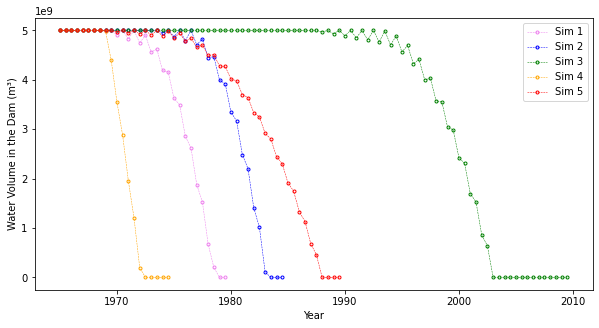
\includegraphics[width=0.9\textwidth]{imagens/model_v0.2.png}
    }\\
    \subfigure[Modelo mensal]{
        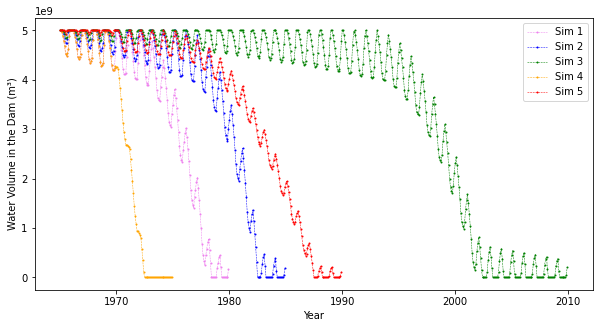
\includegraphics[width=0.9\textwidth]{imagens/model_v1.1.png}
    }\\
    {\flushleft Fonte: os autores. \par}
\end{figure}

\end{document}
